%!TEX root = ../template.tex
%%%%%%%%%%%%%%%%%%%%%%%%%%%%%%%%%%%%%%%%%%%%%%%%%%%%%%%%%%%%%%%%%%%%
%% chapter2.tex
%% NOVA thesis document file
%%
%% Chapter with the template manual
%%%%%%%%%%%%%%%%%%%%%%%%%%%%%%%%%%%%%%%%%%%%%%%%%%%%%%%%%%%%%%%%%%%%

\typeout{NT FILE chapter2.tex}%

\chapter{Background and Related Work}
\label{cha:users_manual}

\glsresetall

%\begin{center}
  %\fbox{\LARGE
  %  This manual is outdated and must be revised!}
%\end{center}

Write something here to introduction to chapter.

\section{Stroke disease}
\label{sec:introduction}

%This Chapter describes how to use the \gls{novathesis}\ template.  It is assumed that you have a working \index{installation} of \LaTeX, either local (in your own computer) or remote (in \Overleaf), and that you were able to generate a PDF for the default configuration of the template: a PhD thesis for \gls{FCT}.
\subsection{Definition}
\label{sec:definitionStroke}
The abrupt onset of a localized neurological deficit caused by a vascular source is the clinical state known as a stroke. This illness is caused by either an internal blood vessel rupture (hemorrhagic stroke) or an obstruction of blood flow to the brain (ischemic stroke). Stroke has a substantial socioeconomic impact and is a leading cause of disability and death worldwide~\cite{Stroke}.

\subsection{Signs and symptoms}
\label{sec:signsandsymptoms}
The portion of the brain affected by a stroke can change the symptoms (see Figure~\ref{fig:Symptoms}). Nonetheless, typical symptoms consist of:
\begin{itemize}
  \item \textbf{Abrupt Weakness or Numbness:} Especially affecting the face, arm, or leg, and usually on one side of the body.
  \item \textbf{Confusion:} Difficulty speaking or understanding speech.
  \item \textbf{Visual Issues:} An abrupt difficulty seeing with one or both eyes.
  \item \textbf{Dizziness and Loss of Coordination:} Sudden trouble walking, dizziness, and loss of balance or coordination.
  \item \textbf{Severe Headache:} An abrupt, intense headache without a recognized reason.
\end{itemize}
Additional symptoms may include difficulty swallowing, difficulty speaking or understanding, abrupt, violent vomiting, or altered awareness~\cite{Stroke,Epidemiologyofstroke}.

\begin{figure}[htbp]
  \centering
  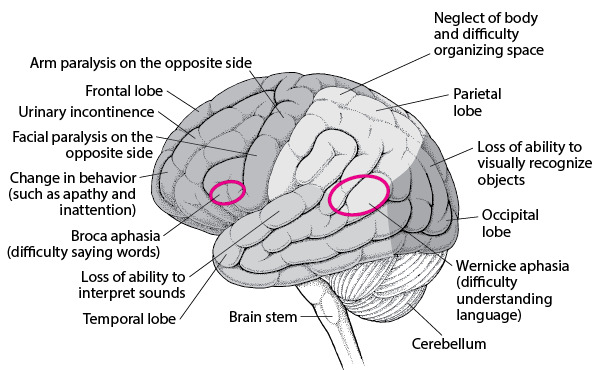
\includegraphics[width=0.75\linewidth]{Symptoms}
  \caption{Areas of the brain affected by a stroke and the specific functions they control~\cite{OverviewofStroke}}\label{fig:Symptoms}
\end{figure}

\subsection{Types of Strokes}
\label{sec:typesofstrokes}
Strokes are broadly classified into two main types: ischemic and hemorrhagic, with a third type, transient ischemic attack (TIA), considered a warning sign.
\begin{enumerate}
  \item \textbf{Ischemic Stroke:}
  As mentioned by Andrei V. Alexandrov and Balaji Krishnaiah~\cite{IschemicStroke}, ``An ischemic stroke typically results from blockage of an artery that supplies blood to the brain, most commonly a branch of one of the internal carotid arteries. As a result, brain cells are deprived of blood. Most brain cells die if they are deprived of blood for 4.5 hours`` (see Figure~\ref{fig:Ischemic_Stroke}). 
  

  Ischemic strokes are further classified into several subtypes based on their etiology~\cite{Stroke}:
  \begin{itemize}
    \item \textbf{Large Artery Atherosclerosis:} Caused by thrombus formation in atherosclerotic vessels, leading to vessel occlusion.
    \item \textbf{Cardioembolic Stroke:} Caused by emboli originating from the heart, often due to atrial fibrillation or other cardiac abnormalities.
    \item \textbf{Small Vessel Occlusion (Lacunar Stroke):} Results from the occlusion of small, penetrating arteries that supply deep brain structures.
    \item \textbf{Cryptogenic Stroke:} An ischemic stroke for which a definitive cause cannot be found despite intensive testing. 
  \end{itemize}
  \begin{figure}[H]
    \centering
    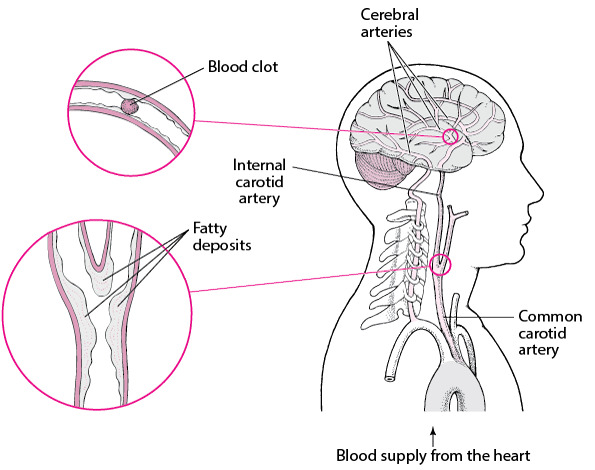
\includegraphics[width=0.7\linewidth]{Ischemic_Stroke}
    \caption{ Illustration of an ischaemic stroke, showing the formation of a blood clot in the internal carotid and cerebral arteries, and fatty deposits that can cause blockage of blood flow to the brain\cite{IschemicStroke}}\label{fig:Ischemic_Stroke}
  \end{figure}

  \item \textbf{Hemorrhagic Stroke:}
  According to Andrei V. Alexandrov and Balaji Krishnaiah~\cite{HemorrhagicStroke}, ``When blood vessels of the brain are weak, abnormal, or under unusual pressure, a hemorrhagic stroke can occur. In hemorrhagic strokes, bleeding may occur within the brain, as an intracerebral hemorrhage. Or bleeding may occur between the inner and middle layer of tissue covering the brain (in the subarachnoid space), as a subarachnoid hemorrhage`` (see Figure~\ref{fig:HemorrhagicStroke}).
  

  Hemorrhagic strokes are further classified into two main types~\cite{Stroke}:
  \begin{itemize}
    \item \textbf{Intracerebral Hemorrhage: } Occurs when a blood vessel within the brain bursts, leading to bleeding into the brain tissue. Common causes include hypertension and cerebral amyloid angiopathy.
    \item \textbf{Subarachnoid Hemorrhage: } Bleeding occurs in the subarachnoid space, often due to ruptured aneurysms or arteriovenous malformations.
  \end{itemize}
  \begin{figure}[H]
    \centering
    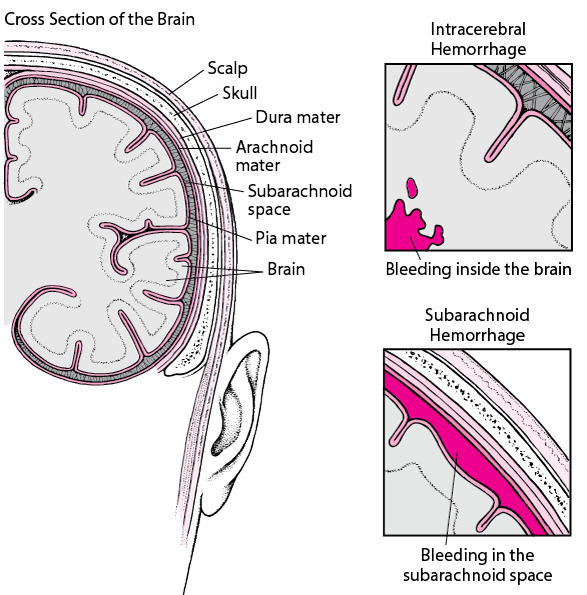
\includegraphics[width=0.7\linewidth]{HemorrhagicStroke}
    \caption{Illustration of a haemorrhagic stroke, showing intracerebral haemorrhage (bleeding inside the brain) and subarachnoid haemorrhage (bleeding in the subarachnoid space)\cite{HemorrhagicStroke}}\label{fig:HemorrhagicStroke}
  \end{figure}
  \item \textbf{Transient Ischemic Attack (TIA):}
  \begin{itemize}
    \item Often called a mini-stroke, a TIA is a temporary period of symptoms similar to those of a stroke. It doesn’t cause permanent damage and is caused by a temporary decrease in blood supply to part of the brain. TIAs are significant predictors of future strokes and should be taken seriously~\cite{Stroke,Epidemiologyofstroke}.
  \end{itemize}
\end{enumerate}




\subsection{Diagnosis}
\label{sec:diagnosisstroke}
Advanced imaging methods and clinical evaluation are combined in the diagnosis of stroke:
\begin{enumerate}
  \item \textbf{Clinical Evaluation:}
\begin{itemize}
  \item To determine the start, nature, and severity of symptoms, a comprehensive history and neurological examination are part of the initial evaluation ~\cite{Epidemiologyofstroke}.
\end{itemize}
\item \textbf{Imaging Methodologies:}
\begin{itemize}
  \item \textbf{Computed Tomography (CT) scan:} The first imaging test used to distinguish between hemorrhagic and ischemic stroke is usually a non-contrast CT scan. It can also aid in ruling out other brain disorders that might resemble the symptoms of a stroke~\cite{Stroke}. 
  \item \textbf{Magnetic Resonance Imaging (MRI):} Provides more detailed images of brain tissue compared to CT scans and is particularly useful in detecting ischemic strokes in the early stages. Diffusion-weighted MRI is more sensitive in detecting early ischemic changes and can help in identifying the exact location and extent of the infarct~\cite{Stroke}.
  \item \textbf{Carotid Ultrasound:} Used to assess blood flow in the carotid arteries and to identify blockages or narrowing that could lead to a stroke~\cite{Stroke}.
  \item \textbf{Cerebral Angiography:} An invasive procedure that involves injecting a contrast dye into the brain's blood vessels to visualize them on X-ray images, helping to identify aneurysms, arteriovenous malformations, and other vascular anomalies~\cite{Stroke1}.
\end{itemize}
\item \textbf{Additional Tests:}
\begin{itemize}
  \item \textbf{Blood Tests:} These may include complete blood count, coagulation profile, and blood glucose levels to identify any underlying conditions that might have contributed to the stroke~\cite{Stroke}.
  \item \textbf{Cardiac Evaluation:} Electrocardiogram (ECG) and echocardiography are used to detect potential cardiac sources of emboli, such as atrial fibrillation or valvular heart disease~\cite{Stroke}.
\end{itemize}  
\end{enumerate}

\subsection{Effects and Complications of Stroke}
\label{sec:effectsofstroke}

\subsection{Treatment}
\label{sec:tretamentstroke}


Thanks to developments in medical technology and our growing understanding of the pathophysiology of strokes, the treatment of strokes has changed dramatically over the past several decades. Stroke therapy options are roughly categorized as acute management, secondary prevention, and rehabilitation. 

\subsubsection{Acute Management}
\label{sec:acutemanagement}
The major goal during the acute phase of stroke treatment is to restore cerebral blood flow as soon as possible. The primary treatment for acute ischemic stroke remains thrombolytic therapy with recombinant tissue plasminogen activator (rt-PA). When given within a short window of 3 to 4.5 hours following the onset of symptoms, rt-PA can considerably lessen neurological damage by dissolving the blood clot clogging the cerebral artery.


However, the use of rt-PA is limited due to rigorous eligibility requirements and the risk of hemorrhagic transformation. As a result, this treatment benefits only a limited number of patients.


In addition to rt-PA, mechanical thrombectomy has become a standard treatment for major vascular occlusions. This procedure involves physically removing the clot with stent retrievers and is most effective when performed within 6 hours of symptom onset~\cite{Therapeuticstrategies}.

\subsubsection{Intensive Stroke Units}
\label{sec:intstrokeunits}
Intensive Stroke Units (ISUs) are a novel approach to stroke therapy, offering patients a dedicated environment in which they get thorough and ongoing care. These units are staffed by a multidisciplinary team of neurologists, nurses, physiotherapists, and occupational therapists, resulting in better patient outcomes such as lower mortality rates and shorter hospital stays~\cite{Treatment_of_stroke_on_an_intensive_stroke_unit}.

\subsubsection{Secondary Prevention}
\label{sec:intstrokeunits}
Preventing recurrent strokes is an important aspect of stroke therapy. This includes addressing modifiable risk factors such hypertension, diabetes, dyslipidemia, and atrial fibrillation. 


Secondary prevention options for cardioembolic stroke include antiplatelet treatment, anticoagulation, and lifestyle adjustments. 


Carotid ultrasonography is commonly used to diagnose carotid artery stenosis, which can be treated surgically by carotid endarterectomy or stenting to lower the risk of future strokes~\cite{Stroke}.

\subsubsection{Rehabilitation}
\label{sec:rehabilitation}
Rehabilitation begins as soon as the patient is medically stable, usually within the first 24-48 hours of hospitalization. A multidisciplinary approach that includes physical therapy, occupational therapy, and speech-language pathology is critical for maximizing functional rehabilitation and encouraging independence. 


The goal of rehabilitation is to improve motor skills, cognitive functions, and everyday activity abilities in stroke survivors, hence improving their overall quality of life ("Treatment of Stroke on an Intensive Stroke Unit: A Novel Concept" by Mohn et al.).

\subsection{Importance of Physiotherapy in Stroke Rehabilitation}
\label{sec:physiotherapy}
Physiotherapy is a critical component of stroke patients rehabilitation, helping them regain function, increase their range of motion, and generally improve their quality of life. 

The process of rehabilitation is intricate and multidimensional, incorporating a range of methods and strategies catered to the individual requirements of every patient.

\subsubsection{Improving Functional Recovery}
\label{sec:improvingfunctionalrecovery}
Physiotherapy's main objective in stroke recovery is to maximize function restoration. To do this, intensive physical treatment is especially beneficial.


Higher intensity physical therapy sessions have been linked to improved functional outcomes, according to studies. 


Compared to patients receiving conventional care, patients receiving more frequent and intensive therapy show considerable increases in mobility and total functional ability ("Physiotherapy After Stroke: More is Better"). 
This emphasizes how crucial it is to offer therapy at a sufficient intensity in order to optimize recovery potential.

\subsubsection{Long-Term Benefits and Persistent Enhancements}
\label{sec:long-termbenefitsandpersistentenhancements}
For stroke survivors, ongoing physiotherapy offers long-term advantages. Sustaining and improving the progress made during the early period of recovery is facilitated by ongoing rehabilitation activities. 


The necessity of ongoing rehabilitation even in the later stages of recovery has been emphasized by meta-analyses that show sustained physiotherapy interventions result in prolonged improvements in physical activity and decreased disability levels ("Efficacy of Physiotherapy Interventions Late After Stroke: A Meta-Analysis"). 

\subsubsection{Neuroplasticity and Recovery}
\label{sec:neuroplasticityandrecovery}
The idea that the brain can rearrange itself by generating new neural connections is known as neuroplasticity, and physiotherapy makes use of this. This is especially crucial for stroke recovery since specific workouts and activities can help restore lost skills and boost brain activity. 


Physiotherapy improves neuroplasticity through targeted, repetitive exercise, which improves recovery ("A Review of Stroke Rehabilitation and Physiotherapy").

\subsubsection{Variety of Techniques and Approaches}
\label{sec:varietyoftechniquesandapproaches}
Various physiotherapy methods support the healing process in different ways. Physiotherapists have embraced the Bobath paradigm, which emphasizes supporting normal movement patterns. Effective stroke rehabilitation practices are built around this strategy and eclectic approaches that incorporate ideas from other ways ("Physiotherapy Treatment for Stroke Patients: A Survey of Current Practice"). 


Furthermore, it has been demonstrated that interventions targeted at increasing physical activity, like exercise training, greatly improve physical fitness and the capacity to carry out everyday tasks ("Efficacy of Interventions Aimmed at Improving Physical Activity in Individuals with Stroke: A Systematic Review").

\section{Self-Management in Stroke Rehabilitation}
\label{sec:selfmanagement}
Escrever aqui alguma coisa  

\subsection{Definition of Self-Management}
\label{sec:definitionofselfmanagement}
Self-management in healthcare refers to the active participation of patients in managing their symptoms, treatments, physical and psychosocial consequences and lifestyle changes associated with chronic illnesses. 


Setting personal goals, monitoring progress, modifying behaviours so that wellbeing can be managed and taking a proactive approach to recovery are all important things that are necessary for people who have survived a stroke. 


Giving patients responsibility for tasks that were previously the responsibility of healthcare professionals gives them the idea that they have more authority and autonomy(Jones, Pöstges,  Brimicombe, Building Bridges Between Healthcare Professionals, Patients, and Families: A Co-Produced and Integrated Approach to Self-Management Support in Stroke).

\subsection{Importance of Self-Management in Stroke Rehabilitation}
\label{sec:importanceofselfmanagement}
Self-management is a fundamental aspect for stroke survivors, having a significant impact on their quality of life and functional independence.


 Appropriate self-management leads to better physical and mental health outcomes, improved functional capabilities and better methods of dealing with long-term effects. It also encourages patients to be more compliant with rehabilitation exercises, thus reducing the risk of complications and reducing the number of hospital readmissions (Lamb et al., Physiotherapy After Stroke: More is Better; Experiences of Self-Management Support Following a Stroke: A Meta-Review of Qualitative Systematic Reviews). 


By taking an active role in their own care, patients are able to achieve better health outcomes and maintain a higher level of independence and quality of life.

\subsection{Elements of effective self-management}
\label{sec:elementesofeffectiveselfmanagement}
Effective self-management programmes for stroke survivors usually include several components:
\begin{itemize}
  \item \textbf{Personalised care plans:}  Consists of adapting rehabilitation plans so that each individual's needs and capabilities are met.
  \item \textbf{Education:} Giving patients all the information about their current condition and explaining the importance of following their rehabilitation plans.
  \item \textbf{Goal Setting:} Helping patients to set realistic and achievable goals that will allow them to recover.
  \item \textbf{Monitoring and feedback:} Regularly assessing the patient's progress and providing constructive feedback to help them stay on track.
  \item \textbf{Problem-solving skills:} Teaching patients strategies to overcome barriers and manage complications independently.
  \item \textbf{Behavioural change:} Encouraging lifestyle changes that support long-term health and recovery.
  \item \textbf{Support systems:} Involve family members and carers to provide both emotional and practical support.(Jones, Pöstges,  Brimicombe, Building Bridges Between Healthcare Professionals, Patients, and Families: A Co-Produced and Integrated Approach to Self-Management Support in Stroke; Strategies for Self-Management Support by Patients with Stroke).
\end{itemize}

\subsection{Autonomy and Social Engagement}
\label{sec:autonomyandsocialengagement}
As well as achieving independence, rehabilitation should also focus on strengthening the patient's autonomy and social involvement. 


Autonomy allows patients to make decisions about their lives, even if they end up needing support to implement them. Social engagement involves building relationships and participating in community activities, which are crucial to the survivor's overall well-being. 


Rehabilitation programmes should aim to balance independence with autonomy and social involvement to improve the quality of life of stroke survivors (Is independence enough? Rehabilitation should include autonomy and social engagement to achieve quality of life).  

\subsection{Obstacles and Difficulties in Self-Management}
\label{sec:ObstaclesandDifficultiesinSelf-Management}
Stroke survivors often face some challenges and obstacles when it comes to self-management. 


Many of them don't feel prepared for the new responsibilities that are thrust upon them. 
The fact that the support systems these survivors have access to are often inadequate makes their self-management efforts more difficult.





















\section{Quick Start}
\label{sec:quick_started}

\subsection{With a Local \LaTeX\ Installation} % (fold)
\label{sub:with_a_local_latex_installation}

Follow these steps to get started with a local \LaTeX\ installation:

\begin{enumerate}
  \item Download \LaTeX.  There are two major \LaTeX\ distributions — \href{https://miktex.org/}{\MikTeX} and \href{https://www.tug.org/texlive/}{\TeXLive} — that share lots of similarity, and \LaTeX\ documents are portable between them. This means that, for most users, both systems are equally usable.
  \begin{description}
    \item [\TeX-Live] is maintained by (La)\TeX\ developers and is certainly the best distribution you may install in your computer:  However, the default distribution will take more than 5\,GB on your hard disk… so, if you are not short on disk space, install \TeXLive!
    \item[Mik\TeX] will, by default, install only a minimal set of packages. The extra/additional packages will be installed on the fly.  Installing packages on the fly is useful if disk space is limited, but has its own caveats in the longer term.  Definitely choose \MikTeX\ if you're short on disk space.
  \end{description}
  Which one to download?  There are \href{https://tex.stackexchange.com/questions/20036/what-are-the-advantages-of-tex-live-over-miktex}{pros and cons for both distributions} so it is essentially a question of where does your heart fall first!  Mine falls to \TeXLive, but yours can fall elsewhere!  \emojiSmile
  \item Install \LaTeX. Installation of \LaTeX\ is as hard as installing any other software.  Just do your best and you will certainly succeed. 
  \item Update your \LaTeX\ installation using the \emph{\TeXLive Utility} program of the \MikTeX\ console.
  \item Download the \gls{novathesis} template by either:
  \begin{itemize}
    \item Cloning the \href{https://github.com/joaomlourenco/novathesis}{GitHub repository} with
    \begin{verbatim}    git clone --depth=1 https://github.com/joaomlourenco/novathesis.git\end{verbatim}
    or
    \item Downloading the \href{https://github.com/joaomlourenco/novathesis/archive/main.zip}{latest version from the GitHub repository as a Zip file}.
  \end{itemize}

  \item \label{it:project_available} Download additional School specific files if applicable:
  \begin{description}
    \item[Universidade do Minho (UMINHO)] download the required \emph{NewsGotT} font files from
    \url{https://github.com/joaomlourenco/novathesis-extras/raw/main/Fonts/NewsGotT.zip}\\
    then unzip the file and copy the~3~font files
\begin{flushleft}
\hspace*{0.5cm}“\verb!n015002t.ttf!”, “\verb!n015003t.ttf!”, and “\verb!n015006t.ttf!”
\end{flushleft}
    to the folder
\begin{flushleft}
\hspace*{0.5cm}“\verb!NOVAthesisFiles/FontStyles/Fonts!”.
\end{flushleft}
    \item[Escola Superior de Enfermagem do Porto (ESEP)] download the required \emph{Calibri} font files from
    \url{https://github.com/joaomlourenco/novathesis-extras/raw/main/Fonts/Calibri.zip}\\
    then unzip the file and copy the~4~font files
\begin{flushleft}
\hspace*{0.5cm}“\verb!Calibri.ttf!”, “\verb!Calibrib.ttf!”, “\verb!Calibrii.ttf!”, and “\verb!Calibriz.ttf!”
\end{flushleft}
      \noindent to the folder
\begin{flushleft}
\hspace*{0.5cm}\verb!NOVAthesisFiles/FontStyles/Fonts!.
\end{flushleft}
  \end{description}

  \item Compile the document with you favorite LaTeX processor (pdfLaTeX, XeLaTeX or LuaLaTeX).
  \begin{itemize}
    \item The main file is named “\verb!template.tex!”, but you are free to rename it as you please.
    \item Either load the main file in your favorite \href{https://en.wikipedia.org/wiki/Comparison_of_TeX_editors}{LaTeX text editor} and press the appropriate (\emph{magic}) button to generate a PDF file, or open a terminal and compile it with “\verb!latexmk -pdf template!”. If you use a \LaTeX\ text editor, please notice that the \gls{novathesis} template uses “\verb!biber!” and not “\verb!bibtex!” to process the bibliography, which means that most probably you have to open the \emph{Editor Preferences} and somewhere (depending on the Editor you are using) change “\verb!bibtex!” to “\verb!biber!”.
    \item Notice that, due to the external font sets used, \pdfLaTeX\ will not work for both \textbf{UMINHO} and \textbf{ESEP}, and you have to use either \XeLaTeX\ (“\verb!latexmk -pdfxe template!”) or \LuaLaTeX (“\verb!latexmk -pdflua template!”).
  \end{itemize}
  \item Edit the files in the “Config” folder:
    \bgroup
    \rowcolors{1}{}{GhostWhite}
    \begin{xltabular}{\textwidth}{>{\ttfamily}lX}
        \toprule
        \rowcolor{Gainsboro}%
        File & Contents \\
        \midrule
0\_memoir.tex       & Options specific for the memoir package. \emph{Don't touch this file unless you know what you are doing!}\\
1\_novathesis.tex   & Configure the template (e.g., the document type, the school, the languages used, etc.)\\
2\_biblatex.tex     & Select how your citations and bibliographic references will be printed.  The default is numbers inside square brackets, e.g. \cite{novathesis-manual}, but you can change it to other formats, such as author-year, e.g., \citeauthor{novathesis-manual}~(\citeyear{novathesis-manual}).\\
3\_cover.tex        & Configure cover contents (e.g., thesis/dissertation title, author's name, advisers' names, committee members' names, date, etc).\\
4\_files.tex        & Select the files for chapters, appendices, annexes, abstracts, glossaries, etc.\\
5\_packages.tex     & User's customization.  Load additional packages and define your own commands to be used throughout the document.\\
6\_list\_of.tex     & Configure the lists to be printed (table of contents, list of figures, list of tables, list of listings, etc). \emph{Don't touch this file unless you know what you are doing!}\\
9\_nova\_fct.tex    & Configuration specific to NOVA-FCT. Otherwise ignored.\\
9\_nova\_ims.tex    & Configuration specific to NOVA-IMS. Otherwise ignored.\\
9\_nova\_itqb.tex   & Configuration specific to NOVA-ITQB. Otherwise ignored.\\
9\_ulisboa\_fmv.tex & Configuration specific to ULISBOA-FMV. Otherwise ignored.\\
9\_uminho.tex       & Configuration specific to UMINHO (all Schools). Otherwise ignored.\\
        \bottomrule
    \end{xltabular}
    \egroup
    % \end{longtblr}
    \item Recompile de document.
    \item And you're done with a beautifully formatted thesis/dissertation! {\setlength{\twemojiDefaultHeight}{1.5\twemojiDefaultHeight}\emojiSmile}
\end{enumerate}

% subsection with_a_local_latex_installation (end)

\subsection{With a Remote Cloud-based Service} % (fold)
\label{sub:with_a_remote_cloud_based_service}

Follow these steps to get started with a remote \LaTeX\ installation:

\begin{itemize}
  \item Download the \href{https://github.com/joaomlourenco/novathesis/archive/main.zip}{latest version from the GitHub repository as a Zip file}.
  \item Login to your favorite LaTeX cloud service. I recommend \href{https://www.overleaf.com/?r=f5160636&rm=d&rs=b}{Overleaf} but there are alternatives. These instructions apply to Overleaf and you'll have to adapt for other providers.
  \item In the menu select \fbox{New project}$\rightarrow$\fbox{Upload project}.
  \item Select “\verb!template.tex!” as the main file.
  \item Follow from Step~\ref{it:project_available} above in Section~\ref{sub:with_a_local_latex_installation} (\nameref{sub:with_a_local_latex_installation}).
\end{itemize}

% subsection with_a_remote_cloud_based_service (end)


\section{Folder and Files}
\label{sec:folders_and_files}

The \gls{novathesis} template is organized into many files and folders. At the main level it includes the following files and folders listed in Table~\ref{tab:folders_and_files}.

\newcommand{\accessAllowed}{\includegraphics[align=c,width=1.9em]{access_allowed}}
\newcommand{\accessForbiden}{\includegraphics[align=c,width=1.9em]{dont_touch}}

\bgroup
    \rowcolors{1}{}{GhostWhite}
      \begin{xltabular}{\textwidth}{>{\ttfamily}l>{\itshape}lcX}
        \caption{The folders and files.}
        \label{tab:folders_and_files}\\
        \toprule
        \rowcolor{Gainsboro}%
        Name & Type & Access & Contents \\
        \midrule
novathesis.cls     & file    & \accessForbiden &
The main class file. %It will include additional files from “\texttt{NOVAthesisFiles}” folder and its sub-folders.
\\
template.tex      & file    & \accessForbiden &
The main template file. You need to \emph{compile} this file with one of \pdfLaTeX, \XeLaTeX, or \LuaLaTeX\ to obtain the PDF file (“\texttt{template.pdf}”).
\\
template.pdf      & file    & \accessAllowed &
A possible result of applying \pdfLaTeX\ to the “\texttt{template.tex}” file. The look and feel of the document will depend on the parametrization/configuration (e.g., School) of this template.
\\
Chapters          & folder  & \accessAllowed &
Examples of document contents, including Chapters, Appendices, Annexes, Abstracts, Glossaries, Lists of Symbols, etc. Replace them with your own.
\\
Bibliography      & folder    & \accessAllowed &
Where all your bibliography files should be located. You may have has many as you want, as long as you add them to the template with “\texttt{\symbol{`\\}ntaddfile\{bib\}\{FILENAME.bib\}}!”. \\
\\
NOVAthesisFiles   & folder  & \accessForbiden &
Additional files for the \gls{novathesis} template.  This is where all the juice is so, unless you are a \TeX magician, don't mess up with the files and folders inside this folder.
\\
        \bottomrule
        \end{xltabular}
    % \end{longtblr}
\egroup

% section folder_structure (end)

% ===================
% = Package options =
% ===================
\section{The \glsfmtshort{novathesisclass}\ Class Options}
\label{sec:package_options}

The \gls{novathesisclass}\ can be customized with the options listed below.

\newcommand{\classoption}[4]{\textbf{#1=OPT}\newline\emph{\small#2}&\textbf{#3}\newline{\small#4}\\}
\newcommand{\defaultopt}[1]{$\Rightarrow$~\emph{Default: \texttt{#1}}\newline}
\newcommand{\defaultit}[1][default]{($\Leftarrow$~\emph{#1})}

\bgroup
  % \rowcolors{1}{}{GhostWhite}
\begin{xltabular}{\linewidth}{>{\hsize=.4\hsize\raggedright\arraybackslash}X>{\hsize=.6\hsize}X}
  \toprule
%----------------------------------------------------------------------
  \classoption{doctype}%
    {phd, phdprop, phdplan, msc, mscplan, bsc, plain}%
    {The type of the document.}{
    \begin{tabular}{@{}r@{ $\rightarrow$ }l@{}}
        phd & PhD thesis \defaultit.\\
    phdprop & PhD thesis proposal (for FCT-NOVA).\\
    phdplan & PhD thesis plan.\\
        msc & MSc dissertation.\\
    mscplan & MSc dissertation plan.\\
        bsc & BSc report.\\
      plain & Other report.\\
    \end{tabular}
    }
    \midrule
%----------------------------------------------------------------------
  \classoption{school}%
    {nova/fct, nova/fcsh, nova/ims, nova/ensp, nova/itqb,\newline ulisboa/ist, ulisboa/fc, ulisboa/fmv,\newline uminho/ea, uminho/ec, uminho/ed, uminho/ee, uminho/eeg, uminho/em, uminho/ep, uminho/ese, uminho/ics, uminho/ie, uminho/elach, uminho/i3b,\newline ips/ests, ipl/isel, ulht/deisi, other/esep}%
    {Selection of the university and of the school.}%
    {\defaultopt{nova/fct} 
     This option changes the typesetting of the de document to some specific School formating and layout, like covers, margins, fonts, paragraph spacing and indentation, etc.}
    \midrule
%----------------------------------------------------------------------
  \classoption{docstatus}%
    {draft, provisional, final}%
    {The current status of the document.}{
    \begin{tabular}{@{}r@{ $\rightarrow$ }X@{}}
         draft        & Working version \defaultit.\\
         provisional  & Version for submission.\\
         final        & Final version.\\
    \end{tabular}
    }
    \midrule
%----------------------------------------------------------------------
  \classoption{lang}%
    {en, pt, de, es, fr, gr, it}%
    {The main language for the document.}{
    \begin{tabular}{@{}l@{ $\rightarrow$ }X@{}}
         en & Enlgish \defaultit.\\
         pt & Portuguese.\\
         de & German.\\
         es & Spanish.\\
         fr & French.\\
         gr & Greek.\\
         it & Italian.\\
    \end{tabular}
    }
    \midrule
%----------------------------------------------------------------------
  \classoption{abstractorder}%
    {\{L$_1$, L$_2$, …, L$_n$\}\newline \{DL=\{L$_1$, L$_2$, …, L$_n$\}\}}%
    {Forces the abstracts languages and order.}{
    \begin{tabular}{@{}l@{ $\rightarrow$ }X@{}}
         DL & Document language \defaultit[defaults to the main language].\\
         L$_i$ & A two-letters language code.\\
    \end{tabular}
    }
    \midrule
%----------------------------------------------------------------------
  \classoption{lang/extra}%
    {\{L$_1$, L$_2$, …, L$_n$\}}%
    {Additional languages used in the document.}{
    \defaultopt{\{\}} 
    Besides the main language and those used in the abstracts.\newline
    \begin{tabular}{@{}l@{ $\rightarrow$ }X@{}}
         L$_i$ & A two-letters language code.\\
    \end{tabular}
    }
    \midrule
%----------------------------------------------------------------------
  \classoption{linkscolor}%
    {A color of your choice.}%
    {The color for all the hyperlinks in the PDF file.}%
    {\defaultopt{darkblue} 
     The “\texttt{media=paper}” option (see below) will override this option to “\texttt{black}”}
    \midrule
%----------------------------------------------------------------------
  \classoption{media}%
    {screen, paper}%
    {The target of the PDF.}%
    {\defaultopt{screen} 
     By default, PDF for screen has colored links and identical left and right margins, while PDF for paper (to print) has black links and may have different left and right margins.}
    \midrule
%----------------------------------------------------------------------
  \classoption{print/index}%
    {true, false}%
    {Produce the document index.}%
    {\defaultopt{false} 
     The index (\emph{índice remissivo}) is a keyword index typeset an the end of the document. WARNING: Should not be confused with the table of contents.}
    \midrule
    
    
    
    
%----------------------------------------------------------------------
  \classoption{fontstyle}%
    {bookman, charter, fourier, kpfonts(*), mathpazo1, mathpazo2, newcent}%
    {The font set to be used in the document.}{Please note that a font set include definitions for the main text, headings, maths, etc.}
    \midrule
%----------------------------------------------------------------------
  \classoption{chapstyle}%
    {bianchi, bluebox, brotherton, dash, default, elegant(*), ell, ger, hansen, ist, jenor, lyhne, madsen, pedersen, veelo, vz14, vz34, vz43}%
    {The chapter style}{The look of the chapter beginning.}
    \midrule
%----------------------------------------------------------------------
  \classoption{converlang}%
    {en, pt(*)}%
    {The language to be used when typesetting the cover page.}{}
    \midrule
%----------------------------------------------------------------------
  \classoption{otherlistsat}%
    {front(*), back}%
    {Where to put the other lists besides the table of contents.}{The default is (\texttt{front}) before the main text.  But some scientific areas prefer them at the end of the document (\texttt{back}), just before the Appendixes.}
    \midrule
%----------------------------------------------------------------------
  \classoption{statement}%
    {true, false(*)}%
    {Include or don't include the contents of the “\texttt{statement}” file.}{The default is for this file to be ignored (if it exists).}
    \midrule
%----------------------------------------------------------------------
  \classoption{spine}%
    {true, false(*)}%
    {Generate the book spine and the last page in the PDF.}{}
    \midrule
%----------------------------------------------------------------------
  \classoption{biblatex}%
    {OPT=\{list of options for \texttt{biblatex}\}}%
    {Customize \texttt{biblatex}, the bibliography management system used in this class.}{Probably you will want to change the value of the \texttt{biblatex} “\texttt{style}” option. For other customizations of \texttt{biblatex} check its manual.}
    \midrule
%----------------------------------------------------------------------
  \classoption{memoir}%
    {OPT=\{list of options for \texttt{memoir}\}}%
    {Customize the base class \texttt{memoir}.}{The \texttt{memoir} manual should be the first document to be consulted when looking for “\textbf{how can I do this?}” You may what to change the base font size from 11pt to a smaller (10pt) or larger (12pt) size.  Also, remember to change the “\texttt{draft}” to final when your document is finished.}
    \midrule
    \bottomrule
\end{xltabular}
\egroup
% \end{ctabular}

\section{Additional considerations about the class options}
\label{sec:additional_considerations}

In this section we will provide some additional considerations about some of the customizations available as class options.

\subsection{The main language}
\label{sub:the_main_language}

The choice of the main language with the option “\texttt{lang=OPT}” affects:

\begin{itemize}
  \item \textbf{The order of the summaries.} First is printed the abstract in the main language and then in the foreign language. This means that if your main language for the document in English, you will see first the “abstract” (in English) and then the “resumo” (in Portuguese). If you switch the main language for the document for Portuguese, it will also automatically switch the order of the summaries to “resumo” and then “abstract”.
  \item \textbf{The names for document sectioning.} E.g., ``Chapter'' vs.\ ``Capítulo'', ``Table of Contents'' vs.\ ``Índice'', ``Figure'' vs.\ ``Figura'', etc.
  \item \textbf{The type of documents in the bibliography.} E.g., ``Technical Report'' vs.\ ``Relatório Técnico'', ``PhD Thesis'' vs.\ ``Tese de Doutoramento'', etc.
\end{itemize}

No mater which language you chose, you will always have the appropriate hyphenation rules according to the language at that point. You always get Portuguese hyphenation rules in the ``Resumo'', English hyphenation rules in the ``Abstract'', and then the main language hyphenation rules for the rest of the document.

% subsection the_main_language (end).

% section additional_consideration (end)


\subsection{Class of Text}
\label{sub:class_of_text}

You must choose the class of text for the document. The available options are:

\begin{enumerate}
  \item \textbf{bsc} --- BSc graduation report.
  \item \textbf{*mscplan} --- Preparation of MSc dissertation. This is a preliminary report graduate students at DI-FCT-NOVA must prepare to conclude the first semester of the two-semesters MSc work. The files specified by \verb!\ntdedicatoryfile! and \verb!\acknowledgmentsfile! are ignored, even if present, for this class of document.
  \item \textbf{msc} --- MSc dissertation.
  \item \textbf{phdprop} ---  Proposal for a PhD work. The files specified by \verb!\ntdedicatoryfile! and \verb!\acknowledgmentsfile! are ignored, even if present, for this class of document.
  \item \textbf{prepphd} ---  Preparation of a PhD thesis. This is a preliminary report PhD students at DI-FCT-NOVA must prepare before the end of the third semester of PhD work. The files specified by \verb!\ntdedicatoryfile! and \verb!\acknowledgmentsfile! are ignored, even if present, for this class of document.
  \item \textbf{phd} --- PhD dissertation.
\end{enumerate}
% subsection class_of_text (end)

% ============
% = Printing =
% ============
\subsection{Printing}
\label{sub:printing}

You must choose how your document will be printed. The available options are:
\begin{enumerate}
  \item \textbf{oneside} --- Single side page printing.
  \item \textbf{*twoside} --- Double sided page printing.
\end{enumerate}
% subsection printing (end)

% =============
% = Font Size =
% =============
\subsection{Font Size}
\label{ssec:font_size}

You must select the encoding for your text. The available options are:
\begin{enumerate}
  \item \textbf{11pt} --- Eleven (11) points font size.
  \item \textbf{*12pt} --- Twelve (12) points font size. You should really stick to 12pt\ldots
\end{enumerate}
% subsection font_size (end)

% =================
% = Text encoding =
% =================
\subsection{Text Encoding}
\label{ssec:text_encoding}

You must choose the font size for your document. The available options are:
\begin{enumerate}
  \item \textbf{latin1} --- Use Latin-1 (\href{http://en.wikipedia.org/wiki/ISO/IEC_8859-1}{ISO 8859-1}) encoding.  Most probably you should use this option if you use Windows;
  \item \textbf{utf8} --- Use \href{http://en.wikipedia.org/wiki/UTF-8}{UTF8} encoding.    Most probably you should use this option if you are not using Windows.
\end{enumerate}
% subsection font_size (end)

% ============
% = Examples =
% ============
\subsection{Examples}
\label{ssec:examples}

Let's have a look at a couple of examples:

\begin{itemize}
  \item Preparation of PhD thesis, in portuguese, with 11pt size and to be printed single sided (I wonder why one would do this!)\\
  \verb!\documentclass[prepphd,pt,11pt,oneside,latin1]{thesisdifct-nova}!
  \item MSc dissertation, in English, with 12pt size and to be printed double sided\\
  \verb!\documentclass[msc,en,12pt,twoside,utf8]{thesisdifct-nova}!
\end{itemize}
% subsection examples (end)

\section{How to Write Using \LaTeX}
\label{sec:how_to_write_using_latex}

Please have a look at Chapter~\ref{cha:a_short_latex_tutorial_with_examples}, where you may find many examples of \LaTeX constructs, such as Sectioning, inserting Figures and Tables, writing Equations, Theorems and algorithms, exhibit code listings, etc.

% section how_to_write_using_latex (end)



\section{Example glossary, acronyms, and symbols}
%
% \todo[inline]{A a note in a line by itself.}
%
This is the first occurrence of an abbreviation: \gls{abbrev}. And now the second occurrence of the same abbreviation: \gls{abbrev}. And a new acronym with capital letter: \Gls{xpt} and reused \gls{xpt}.  Let's also use a few other acronyms such as \gls{aaa}, \gls{aab}, \gls{aba}, \gls{bbb} and \gls{xpt}.
In geometry, the area enclosed by a circle of radius \gls{r} is $\pi r^2$. Here the Greek letter \gls{pi} is equal to the ratio of the circumference of any circle to its diameter.
Lets add ``\gls{computer}'' to the glossary! Be carefull with mathematical symbols in acronyms, please see the definition of \gls{mu}.

% Reference to Potassium \gls{chem:potassio} and Sodium \gls{chem:sodio} as well.

%
% Please note that
% \begin{center}
%   \textbf{\large this package and template are not official for FCT/NOVA}.
% \end{center}



% \printbibliography[heading=subbibliography, segment=\therefsegment, title={\bibname\ for chapter~\thechapter}]


\endinput

%!TEX root = ../template.tex
%%%%%%%%%%%%%%%%%%%%%%%%%%%%%%%%%%%%%%%%%%%%%%%%%%%%%%%%%%%%%%%%%%%%
%% chapter2.tex
%% NOVA thesis document file
%%
%% Chapter with the template manual
%%%%%%%%%%%%%%%%%%%%%%%%%%%%%%%%%%%%%%%%%%%%%%%%%%%%%%%%%%%%%%%%%%%%

\typeout{NT FILE chapter2.tex}%

\chapter{NOVAthesis Template \emph{User's Manual}}
\label{cha:users_manual}

\glsresetall

\begin{center}
  \fbox{\LARGE
    This manual is outdated and must be revised!}
\end{center}

Referência ao Potássio é \gls{chem:potassio} e Sódio também \gls{chem:sodio}.

\section{Introduction}
\label{sec:introduction}

This chapter describes how to use the \gls{novathesis}\ Template and the \gls{novathesisclass} file.  I will assume you have a working installation of \LaTeX, wither local (in your own computer) or remote (in Overleaf), and that it compiled successfully the default configuration (PhD for \gls{FCT}).


\section{Folder Structure}
\label{sec:folder_structure}

The \gls{novathesis} template is organized into many files and folders. At the main level it includes the following files and folders:

\noindent
\bgroup
\rowcolors{1}{GhostWhite}{}
\begin{xltabular}{\linewidth}{>{\ttfamily}l>{\itshape}l>{\upshape}X}
novathesis.cls     & file    &
The main class file. It will include additional files from \texttt{NOVAthesisFiles} folder and its sub-folders.
\\
template.tex      & file    &
The main template file. You need to \emph{compile} this file with one of pdf\LaTeX, \XeLaTeX, or \LuaLaTeX\ to obtain the \texttt{template.pdf} file.
\\
bibliography.bib  & file    &
An example of a bibliography file. You may have has many as you want. \\
template.pdf      & file    &
A possible result of applying pdf\LaTeX\ to the \texttt{template.tex} file. The template supports multiple types of documents (e.g., MSc dissertation, PhD thesis, …) and multiple Schools (e.g., FCT-NOVA, FCSH-NOVA, IST-UL, FC-UL, …) and each will produce different results.
\\
Chapters          & folder  & Examples of thesis chapters. Replace them with your own chapters.
\\
Examples          & folder  & Some more examples of the use of the template for different document types and Schools.
\\
Scripts           & folder  & Some (possibly useful) scripts for Unix-based systems (Linux, Mac OSx). If you are a windows user, ignore this folder (you may safely delete it if you want).
\\
NOVAthesisFiles   & folder  &
Additional files for the \gls{novathesisclass}\ file.  Unless you know what you are doing, avoid messing up with the files and folders inside this folder (except for deleting the unused Schools, see below).
\\
\end{xltabular}
\egroup

The \texttt{NOVAthesisFiles} folder contains additional files and folders that complement the main \gls{novathesisclass}\ file.  These are:

\noindent
\bgroup
\rowcolors{1}{GhostWhite}{}
\begin{tabularx}{\linewidth}{>{\ttfamily}l>{\itshape}l>{\upshape}X}
README.txt      & file    &
A file that should be read!  :)
\\
fix-babel.tex   & file    &
Simple fixes to the \texttt{babel} package.
\\
lang-text.ldf   & file    &
Translations of important strings used in the template.  Currently fully supported are Portuguese and English, but French is on the way.  If you add translations for your own language, please be so kind and send them to me. Thank you!
\\
options.tex     & file    &
Processing of \gls{novathesisclass}\ options.  \emph{Don't mess with this!}
\\
packages.tex    & file    &
Additional packages to be loaded into the \gls{novathesis}\ template. \emph{You should not mess with this!}
\\
spine.tex       & file    &
This file is loaded only if the option \texttt{spine=full} or \texttt{spine=trim}, and includes the typesetting of the book spine.
\\
ChapStyles      & folder  &
Contains a lot of files, one for each chapter style.  If you really know what you are doing, you may add your own chapter style here.
\\
FontStyles      & folder  &
Contains a few files, one for each set of fonts (main text font, chapter font, section font, subsection font, etc).  If you really know what you are doing, you may add your own set here.
\\
Schools         & folder  &
Configuration files for each school.  This folder is organized into subfolders, one for each university.  \emph{You may safely delete all the subfolders except the one for your University.}  Then open the subfolder of your University and \emph{you may safely delete all the subfolders except the one for your School/Faculty}.
\\
\end{tabularx}
\egroup

As stated above, the \texttt{Schools} folder contains per-university folders and per-school (faculty) subfolders.  Currently these are the available folders:

\noindent
\bgroup
\rowcolors{1}{GhostWhite}{}
\begin{tabularx}{\linewidth}{>{\ttfamily}r@{~/~}>{\ttfamily}l>{\itshape}l>{\upshape}X}
ul     & ist    & folder  &
The folder for the \href{http://www.tecnico.ulisboa.pt}{\emph{Instituto Superior Técnico}} of the \emph{University of Lisbon}.
\\
nova    & fcsh   & folder  &
The folder for the \href{http:www.fcsh.unl.pt}{\emph{Faculty of Human and Social Sciences}}  of the \emph{NOVA University of Lisbon}.
\\
nova    & fct    & folder  &
The folder for the \href{http:www.fct.unl.pt}{\emph{Faculty of Sciences and Technology}} of the \emph{NOVA University of Lisbon}.
\\
nova    & novaims    & folder  &
The folder for the \href{http:www.novaims.unl.pt}{\emph{Information and Management School}} of the \emph{NOVA University of Lisbon}.
\\
\end{tabularx}
\egroup

% section folder_structure (end)

% ===================
% = Package options =
% ===================
\section{\glsfmtshort{novathesisclass}\ Class Options}
\label{sec:package_options}

The \gls{novathesisclass}\ can be customized with the options listed below.

\newcommand{\classoption}[3]{\textbf{#1=OPT}\qquad #2\\\qquad\emph{#3}\\}

\noindent
\begin{ctabular}{@{}p{\linewidth}@{}}
  \toprule
%----------------------------------------------------------------------
  \classoption{doctype}%
    {phd(*), phdplan, phdprop, msc, mscplan, bsc}%
    {The type of the document: PhD Thesis (---~Default~---), PhD Plan, PhD Proposal, MSc Dissertation, MSc Plan, BSc Report}
    \midrule
%----------------------------------------------------------------------
  \classoption{school}%
    {nova/fct(*), nova/fcsh, nova/ims, ul/ist, ul/fc}%
    {The name of the school. This option changes the typesetting of the cover and some School specific formating, like margins, fonts, paragraph spacing and indentation, etc…}
    \midrule
%----------------------------------------------------------------------
  \classoption{lang}%
    {en(*), pt}%
    {The main language for the document.  Currently only Portuguese and English are supported.  Other languages are expected to be support in forthcoming versions.}
    \midrule
%----------------------------------------------------------------------
  \classoption{fontstyle}%
    {bookman, charter, fourier, kpfonts(*), mathpazo1, mathpazo2, newcent}%
    {The font set to be used in the document.  Please note that a font set include definitions for the main text, headings, maths, etc.}
    \midrule
%----------------------------------------------------------------------
%----------------------------------------------------------------------
  \classoption{chapstyle}%
    {bianchi, bluebox, brotherton, dash, default, elegant(*), ell, ger, hansen, ist, jenor, lyhne, madsen, pedersen, veelo, vz14, vz34, vz43}%
    {The chapter style, i.e., the look of the chapter beginning.}
    \midrule
%----------------------------------------------------------------------
  \classoption{converlang}%
    {en, pt(*)}%
    {The language to be used when typesetting the cover page.}
    \midrule
%----------------------------------------------------------------------
  \classoption{otherlistsat}%
    {front(*), back}%
    {Where to put the other lists besides the table of contents. The default is (\texttt{front}) before the main text.  But some scientific areas prefer them at the end of the document (\texttt{back}), just before the Appendixes.}
    \midrule
%----------------------------------------------------------------------
  \classoption{statement}%
    {true, false(*)}%
    {Include or don't include the contents of the “\texttt{statement}” file. The default is for this file to be ignored (if it exists).}
    \midrule
%----------------------------------------------------------------------
  \classoption{linkscolor}%
    {darkblue(*), black}%
    {The color for all the hyperlinks in the PDF file.  The “\texttt{media=paper}” option (see below) will override this option to “\texttt{black}”}
    \midrule
%----------------------------------------------------------------------
  \classoption{spine}%
    {true, false(*)}%
    {Generate the book spine and the last page in the PDF.}
    \midrule
%----------------------------------------------------------------------
  \classoption{biblatex}%
    {OPT=\{list of options for \texttt{biblatex}\}}%
    {Customize \texttt{biblatex}, the bibliography management system used in this class. Probably you will want to change the value of the \texttt{biblatex} “\texttt{style}” option. For other customizations of \texttt{biblatex} check its manual.}
    \midrule
%----------------------------------------------------------------------
  \classoption{memoir}%
    {OPT=\{list of options for \texttt{memoir}\}}%
    {Customize the base class \texttt{memoir}. The \texttt{memoir} manual should be the first document to be consulted when looking for “\textbf{how can I do this?}” You may what to change the base font size from 11pt to a smaller (10pt) or larger (12pt) size.  Also, remember to change the “\texttt{draft}” to final when your document is finished.}
    \midrule
%----------------------------------------------------------------------
  \classoption{media}%
    {screen(*), paper}%
    {Behavior to be customized in the school options/configuration. Expected definitions for screen are: left and right margins are equal and use colored links. Expected definitions for paper are: left and right margins are different and use black links.}
    \bottomrule
\end{ctabular}

\section{Additional considerations about the class options}
\label{sec:additional_considerations}

In this section we will provide some additional considerations about some of the customizations available as class options.

\subsection{The main language}
\label{sub:the_main_language}

The choice of the main language with the option “\texttt{lang=OPT}” affects:

\begin{itemize}
  \item \textbf{The order of the summaries.} First is printed the abstract in the main language and then in the foreign language. This means that if your main language for the document in English, you will see first the “abstract” (in English) and then the “resumo” (in Portuguese). If you switch the main language for the document for Portuguese, it will also automatically switch the order of the summaries to “resumo” and then “abstract”.
  \item \textbf{The names for document sectioning.} E.g., ``Chapter'' vs.\ ``Capítulo'', ``Table of Contents'' vs.\ ``Índice'', ``Figure'' vs.\ ``Figura'', etc.
  \item \textbf{The type of documents in the bibliography.} E.g., ``Technical Report'' vs.\ ``Relatório Técnico'', ``PhD Thesis'' vs.\ ``Tese de Doutoramento'', etc.
\end{itemize}

No mater which language you chose, you will always have the appropriate hyphenation rules according to the language at that point. You always get Portuguese hyphenation rules in the ``Resumo'', English hyphenation rules in the ``Abstract'', and then the main language hyphenation rules for the rest of the document.

% subsection the_main_language (end).

% section additional_consideration (end)


\subsection{Class of Text}
\label{sub:class_of_text}

You must choose the class of text for the document. The available options are:

\begin{enumerate}
  \item \textbf{bsc} --- BSc graduation report.
  \item \textbf{*mscplan} --- Preparation of MSc dissertation. This is a preliminary report graduate students at DI-FCT-NOVA must prepare to conclude the first semester of the two-semesters MSc work. The files specified by \verb!\ntdedicatoryfile! and \verb!\acknowledgmentsfile! are ignored, even if present, for this class of document.
  \item \textbf{msc} --- MSc dissertation.
  \item \textbf{phdprop} ---  Proposal for a PhD work. The files specified by \verb!\ntdedicatoryfile! and \verb!\acknowledgmentsfile! are ignored, even if present, for this class of document.
  \item \textbf{prepphd} ---  Preparation of a PhD thesis. This is a preliminary report PhD students at DI-FCT-NOVA must prepare before the end of the third semester of PhD work. The files specified by \verb!\ntdedicatoryfile! and \verb!\acknowledgmentsfile! are ignored, even if present, for this class of document.
  \item \textbf{phd} --- PhD dissertation.
\end{enumerate}
% subsection class_of_text (end)

% ============
% = Printing =
% ============
\subsection{Printing}
\label{sub:printing}

You must choose how your document will be printed. The available options are:
\begin{enumerate}
  \item \textbf{oneside} --- Single side page printing.
  \item \textbf{*twoside} --- Double sided page printing.
\end{enumerate}
% subsection printing (end)

% =============
% = Font Size =
% =============
\subsection{Font Size}
\label{ssec:font_size}

You must select the encoding for your text. The available options are:
\begin{enumerate}
  \item \textbf{11pt} --- Eleven (11) points font size.
  \item \textbf{*12pt} --- Twelve (12) points font size. You should really stick to 12pt\ldots
\end{enumerate}
% subsection font_size (end)

% =================
% = Text encoding =
% =================
\subsection{Text Encoding}
\label{ssec:text_encoding}

You must choose the font size for your document. The available options are:
\begin{enumerate}
  \item \textbf{latin1} --- Use Latin-1 (\href{http://en.wikipedia.org/wiki/ISO/IEC_8859-1}{ISO 8859-1}) encoding.  Most probably you should use this option if you use Windows;
  \item \textbf{utf8} --- Use \href{http://en.wikipedia.org/wiki/UTF-8}{UTF8} encoding.    Most probably you should use this option if you are not using Windows.
\end{enumerate}
% subsection font_size (end)

% ============
% = Examples =
% ============
\subsection{Examples}
\label{ssec:examples}

Let's have a look at a couple of examples:

\begin{itemize}
  \item Preparation of PhD thesis, in portuguese, with 11pt size and to be printed single sided (I wonder why one would do this!)\\
  \verb!\documentclass[prepphd,pt,11pt,oneside,latin1]{thesisdifct-nova}!
  \item MSc dissertation, in English, with 12pt size and to be printed double sided\\
  \verb!\documentclass[msc,en,12pt,twoside,utf8]{thesisdifct-nova}!
\end{itemize}
% subsection examples (end)

\section{How to Write Using \LaTeX}
\label{sec:how_to_write_using_latex}

Please have a look at Chapter~\ref{cha:a_short_latex_tutorial_with_examples}, where you may find many examples of \LaTeX constructs, such as Sectioning, inserting Figures and Tables, writing Equations, Theorems and algorithms, exhibit code listings, etc.

% section how_to_write_using_latex (end)



\section{Example glossary, acronyms, and symbols}
%
% \todo[inline]{A a note in a line by itself.}
%
This is the first occurrence of an abbreviation: \gls{abbrev}. And now the second occurrence of the same abbreviation: \gls{abbrev}. And a new acronym with capital letter: \Gls{xpt} and reused \gls{xpt}.  Let's also use a few other acronyms such as \gls{aaa}, \gls{aab}, \gls{aba}, \gls{bbb} and \gls{xpt}.
In geometry, the area enclosed by a circle of radius \gls{r} is $\pi r^2$. Here the Greek letter \gls{pi} is equal to the ratio of the circumference of any circle to its diameter.
Lets add ``\gls{computer}'' to the glossary! Be carefull with mathematical symbols in acronyms, please see the definition of \gls{mu}.
%
% Please note that
% \begin{center}
%   \textbf{\large this package and template are not official for FCT/NOVA}.
% \end{center}



% \printbibliography[heading=subbibliography, segment=\therefsegment, title={\bibname\ for chapter~\thechapter}]
